
\documentclass[11pt, a4paper]{book}
\usepackage{svn-multi}
\svnid{$Id$}
\usepackage{latexsym}
\usepackage{prelim2e}
\renewcommand{\PrelimWords}{Draft Copy \svnkw{Id}}
%%\newcommand*{\mysvnrev}{\svnrev}
\usepackage[hyperindex=true,
			bookmarks=true,
            pdftitle={}, pdfauthor={Xi Yang},
            colorlinks=false,
            pdfborder=0,
            pagebackref=false,
            citecolor=blue,
            plainpages=false,
            pdfpagelabels,
            pagebackref=true,
            hyperfootnotes=false]{hyperref}
\usepackage[all]{hypcap}
\usepackage[palatino]{anuthesis}
\usepackage{afterpage}
\usepackage{graphicx}
\usepackage{thesis}
\usepackage[square]{natbib}
\usepackage[normalem]{ulem}
\usepackage[table]{xcolor}
\usepackage{makeidx}
\usepackage{cleveref}
\usepackage[justification=justified,singlelinecheck=false]{caption}
\usepackage{float}
\urlstyle{sf}
\renewcommand{\sfdefault}{uop}
\usepackage[T1]{fontenc}
\usepackage[scaled]{beramono}

\usepackage{multirow}
\usepackage{algorithm}
\usepackage{algorithmic}
\usepackage{tikz}
\usepackage{amsmath}

\renewcommand*{\backref}[1]{}
\renewcommand*{\backrefalt}[4]{
  \ifcase #1 %
    %
  \or
    (cited on page #2)%
  \else
    (cited on pages #2)%
  \fi
} 


%      $Id: macros.tex 506 2009-10-05 16:57:07Z daniel $    

\usepackage{booktabs}
\usepackage{relsize}
\usepackage{xspace}
\usepackage{subfigure}
\usepackage{listings}
\lstloadlanguages{java}
\DeclareGraphicsRule{*}{pdf}{*}{}
\newcommand{\otoprule}{\midrule[\heavyrulewidth]}
\newcommand{\pldi}{ACM Programming Language Design and Implementation (PLDI)}
\newcommand{\taco}{ACM Transactions on Architecture and Code Optimization (TACO)}
\newcommand{\lctes}{ACM Languages, Compiler, and Tool Support for Embedded Systems (LCTES)}
\newcommand{\popl}{ACM Principles of Programming Languages (POPL)}
\newcommand{\ecoop}{European Conference for Object-Oriented Programming (ECOOP)}
\newcommand{\asplos}{ACM Architectural Support for Programming Languages and Operating Systems (ASPLOS)}
\newcommand{\sigmetrics}{ACM Measurement and Modeling of Computer Systems (SIGMETRICS)}
\newcommand{\oopsla}{ACM Object-Oriented Programming, Systems, Languages, and Applications (OOPSLA)}
\newcommand{\ismm}{International Symposium on Memory Management (ISMM)}
\newcommand{\veee}{ACM/USENIX Virtual Execution Environments (VEE)}
\newcommand{\micro}{ACM/IEEE International Symposium on Microarchitecture}
\newcommand{\isca}{ACM/IEEE International Symposium on Computer Architecture (ISCA)}
\newcommand{\icse}{International Conference  on Software Engineering (ICSE)}
\newcommand{\pact}{Parallel Architectures and Compilation Techniques (PACT)}
\newcommand{\casess}{ACM Compilers, Architectures, and Synthesis for Embedded Systems (CASES)}

\definecolor{tableheadcolor}{rgb}{0.8,0.8,1.0}
%\definecolor{tablealtcolor}{rgb}{0.9,0.9,1.0}
\definecolor{tablealtcolor}{rgb}{0.9,0.9,0.95}


\definecolor{todocolor}{rgb}{0.8,0.8,1.0}
\definecolor{fixcolor}{rgb}{1,0.8,0.8}
\definecolor{commentcolor}{rgb}{0.8,1.0,0.8}


\newcommand{\listingfigure}[3]{
\begin{figure}[ht!]
  \begin{center}
    \begin{minipage}[t]{\textwidth-4cm}
      \lstinputlisting{#1}
    \end{minipage}
  \end{center}
  \caption{#3}#2
\end{figure}}

\newcommand{\includeabchart}[5]{
\begin{figure}[ht!]
\begin{center}
\newcommand{\atitle}{#4}
\newcommand{\btitle}{#5}
\input{charts/#1.tex}
\end{center}
\caption{#3}#2
\end{figure}}

\newcommand{\placeholderfigure}[2]{
\begin{figure}[ht!]
  \begin{center}
    \resizebox{\textwidth-2cm}{0.7\textwidth-1.4cm}{todo}
  \end{center}
  \caption{#2}#1
\end{figure}}

\newcommand{\singlegraphfigure}[3]{
\begin{figure}[ht!]
  \begin{center}
    \includegraphics[width=\textwidth-2cm]{#1}
  \end{center}
  \caption{#3}#2
\end{figure}}

\usepackage[color=todocolor, colorinlistoftodos]{todonotes}

%\newcommand{\notinpart}{%
% \def\toclevel@chapter{-1}\def\toclevel@section{0}\def\toclevel@subsection{1}} \newcommand{\inpart}{
% \def\toclevel@chapter{0}\def\toclevel@section{1}\def\toclevel@subsection{2}}


%
% Stuff for pretty printing the source code using listings.sty
%


%% set Java as the default language
\lstset{
  numbers=left,
  numberstyle=\tiny,
  stepnumber=1,
  numbersep=2em,
  language=java,                         % the language
  basicstyle=\footnotesize\ttfamily,     % the basic font family to use
  commentstyle=\itshape,                 % the font for comments
  stringstyle=\ttfamily,
%  morekeywords={@Intrinsic, @Unboxed, @RawStorage}
}
%\lstset{language=java}

\newcommand{\textjava}[1]{{\lstset{basicstyle=\ttfamily}\lstinline@#1@}}
\newcommand{\textjavafn}[1]{{\lstset{basicstyle=\footnotesize\ttfamily}\lstinline@#1@}}
%\usepackage{lstasm}
\usepackage{setspace}
\usepackage{ifthen}
%\usepackage{color}
%\usepackage{smallheadings}

\long\def\sfootnote[#1]#2{\begingroup%
\def\thefootnote{\fnsymbol{footnote}}\footnote[#1]{#2}\endgroup}
%
% code
%

\newcommand{\address}{\textjava{Address}\xspace}
\newcommand{\ubregion}{\textjava{unbump-region()}\xspace}
\newcommand{\word}{\textjava{Word}\xspace}
\newcommand{\freeme}{\textjava{free()}\xspace}
\newcommand{\freemeunbump}{\textjava{unbump()}\xspace}
\newcommand{\freemeunbumpregion}{\textjava{unbump-region()}\xspace}
\newcommand{\freemeunreserve}{\textjava{unreserve()}\xspace}

%
% abbreviations
%


\newcommand{\eg}{e.g., }
\newcommand{\ie}{i.e., }

\newcommand{\GenMS}{\emph{GenMS}\xspace}
\newcommand{\GenImmix}{\emph{GenIX}\xspace}
\newcommand{\mmtk}{MMTk\xspace}
\newcommand{\jikes}{Jikes RVM\xspace} 
\newcommand{\jikesrvm}{\jikes} 
\newcommand{\jala}{Jalape\~{n}o\xspace} 
\newcommand{\jalapeno}{Jalape\~{n}o\xspace} 

\newcommand{\dacapo}{\textsf{DaCapo}\xspace}
\newcommand{\specjvm}{\textsf{SPECjvm98}\xspace}
\newcommand{\cattrack}{\textsf{cattrack}\xspace}
\newcommand{\spec}{\textsf{SPEC}\xspace}

\newcommand{\nurserytype}[1]{{\fontfamily{cmss}\selectfont \textsl{#1}}}
\newcommand{\alloc}{\nurserytype{allocate}\xspace}
\newcommand{\collect}{\nurserytype{collect}\xspace}
\newcommand{\redirect}{\nurserytype{redirect}\xspace}

\newcommand{\bmtype}[1]{{\textsf{#1}}}

\newcommand{\jbb}{\bmtype{jbb2000}\xspace}
\newcommand{\psjbb}{\bmtype{pjbb2005}\xspace}
\newcommand{\pjbb}{\bmtype{pjbb2005}\xspace}
\newcommand{\specjbb}{\bmtype{SPECjbb2005}\xspace}
\newcommand{\jess}{\bmtype{jess}\xspace}
\newcommand{\raytrace}{\bmtype{raytrace}\xspace}
\newcommand{\db}{\bmtype{db}\xspace}
\newcommand{\javac}{\bmtype{javac}\xspace}
\newcommand{\jack}{\bmtype{jack}\xspace}
\newcommand{\compress}{\bmtype{compress}\xspace}
\newcommand{\mpegaudio}{\bmtype{mpegaudio}\xspace}
\newcommand{\mtrt}{\bmtype{mtrt}\xspace}
\newcommand{\antlr}{\bmtype{antlr}\xspace}
\newcommand{\bloat}{\bmtype{bloat}\xspace}
\newcommand{\chart}{\bmtype{chart}\xspace}
\newcommand{\eclipse}{\bmtype{eclipse}\xspace}
\newcommand{\fop}{\bmtype{fop}\xspace}
\newcommand{\hsqldb}{\bmtype{hsqldb}\xspace}
\newcommand{\jython}{\bmtype{jython}\xspace}
\newcommand{\luindex}{\bmtype{luindex}\xspace}
\newcommand{\lusearch}{\bmtype{lusearch}\xspace}
\newcommand{\Lusearch}{\bmtype{Lusearch}\xspace}
\newcommand{\pmd}{\bmtype{pmd}\xspace}
\newcommand{\ps}{\bmtype{ps}\xspace}
\newcommand{\SPECjbb}{\bmtype{SPECjbb}\xspace}
\newcommand{\xalan}{\bmtype{xalan}\xspace}
\newcommand{\sunflow}{\bmtype{sunflow}\xspace}
\newcommand{\Sunflow}{\bmtype{Sunflow}\xspace}
\newcommand{\avrora}{\bmtype{avrora}\xspace}
\newcommand{\core}{Core2 Quad\xspace}
\newcommand{\corelong}{Intel Core2 Quad Q6600\xspace}
\newcommand{\phenom}{Phenom II\xspace}
\newcommand{\phenomlong}{AMD Phenom II X6 1055T\xspace}
\newcommand{\sandy}{i7-2600\xspace}
\newcommand{\sandylong}{Intel Core i7-2600\xspace}



\newcommand{\ghostscript}{\bmtype{ghostscript}\xspace}

\newcommand{\doi}[1]{\href{http://dx.doi.org/#1}{\nolinkurl{doi:#1}}}
%
% misc
%
\newcommand{\fix}[1]{\todo[color=fixcolor]{#1}}
\newcommand{\comment}[1]{\todo[color=commentcolor]{#1}}
\newcommand{\ifix}[1]{\todo[inline,color=fixcolor]{#1}}
\newcommand{\icomment}[1]{\todo[inline,color=commentcolor]{#1}}
\newcommand{\itodo}[1]{\todo[inline]{#1}}
\newcommand{\ignore}[1]{}
\newcommand{\mccenter}[1]{\multicolumn{1}{c|}{#1}}

%
% figure spacing
%
%\clubpenalty 10000
%\widowpenalty 10000
%\def\topfraction{0.9}
%\def\bottomfraction{0.9}
%\def\textfraction{0.1}
%\renewcommand{\singlespacing}{\renewcommand{\baselinestretch}{1.00}\small\normalsize}
%\renewcommand{\doublespacing}{\renewcommand{\baselinestretch}{1.5}\small\normalsize}
%\newcommand{\tight}{\renewcommand{\baselinestretch}{1.28}\small\normalsize}
%\renewcommand{\subfigbottomskip}{0.25ex}
%\renewcommand{\subfigcapskip}{0ex}
%\renewcommand{\subfigcapskip}{-1ex}
%\newcommand{\subfigshrink}{-0.75ex}
%\newcommand{\subfigcapspace}{2ex}

%\newcommand{\subwidth}[0]{.32\textwidth}


%
% margins
%
%\topmargin -.5truein
%\textheight 9truein
%\oddsidemargin .25truein
%\evensidemargin .25truein
%\textwidth 6truein


%
% crossreferencing footnotes
%
%\newcommand{\fnref}[1]{~(\ref{#1})}
%\newcommand{\onecolparbox}{3.1in}


%\newcommand{\textjava}[1]{{\lstset{language=java,basicstyle=\footnotesize\ttfamily}\lstinline@#1@}}
%\newcommand{\textasm}[1]{{\lstset{language=asm,basicstyle=\footnotesize\ttfamily}\lstinline@#1@}}

%%
%% Change the sections etc.
%%
%\makeatletter
%\parskip=0pt
%\renewcommand\section{\@startsection{section}{1}{\z@}%
%                                   {-2.5ex}% beforeskip
%%                                   {1ex}% afterskip
%                                   {\large \bfseries \raggedright}}
% \renewcommand\subsection{\@startsection{subsection}{2}{\z@}%
%                                     {-2ex\@plus -1ex \@minus -.2ex}%
%                                      {.5ex \@plus .2ex}%
%                                      {\normalsize \bfseries \raggedright}}
% \renewcommand\subsubsection{\@startsection{subsubsection}{3}{\z@}%
%                                      {-2ex\@plus -1ex \@minus -.2ex}%
%                                      {1ex \@plus .2ex}%
%                                      {\normalfont\fontsize{11pt}{12pt}\selectfont\itshape}}
%\renewcommand{\thesubsubsection}{\thesubsection.\arabic{subsubsection}}

%\renewcommand\paragraph{\@startsection{paragraph}{4}{\z@}% 
%  {.5em}%
%  {-1em}%
%  {\normalfont\normalsize\bfseries\parskip=0pt}}
%\setlength\partopsep{0\p@}
%\setlength\parskip{0\p@ \@plus \p@}

%\makeatother
%\parindent=9pt





%%% Local Variables: 
%%% mode: latex
%%% TeX-master: "doa"
%%% End:
            
%%%%%%%%%%%%%%%%%%%%%%%%%%%%%%%%%%%%%%%%%%%%%%%%%%%%%%%%%%%%%%%%%%%%%%%
%% Preamble
\title{Fast and Optimal Pathfinding in Symmetric Domains}
\author{Daniel Harabor}
\date{\today}

\renewcommand{\thepage}{\roman{page}}

\newtheorem{theorem}{Theorem}
\newtheorem{lemma}{Lemma}
\newtheorem{proposition}{Proposition}
\newtheorem{corollary}{Corollary}
\newtheorem{definition}{Definition}
\newenvironment{proof}{\noindent{\bf Proof:}}{\hspace{\stretch{1}}$\Box$\vspace{0.5em}\newline}

\newcommand{\figref}[1]{\figurename~\ref{#1}}
\newenvironment{pth}{\langle}{\rangle}

\usetikzlibrary{intersections}
\newcommand{\intersection}[2]{\langle #1, #2\rangle}
\newcommand{\anya}[0]{{\bf anya}}
\newcommand{\creategrid}[2]{%
  \draw[step=1] (0,0) grid (#1,#2);%
%
  \foreach \x in {1,...,#1}%
    \draw (\x - 0.5, -0.5) node {\x};%
%
  \foreach \y in {1,...,#2}%
    \draw (-0.5, \y - 0.5) node {\y};%
}%
\newcommand{\drawobstacle}[2]{%
\draw[fill=black] (#1,#2) rectangle +(-1,-1);
}%


\DeclareMathOperator*{\argmin}{arg\,min}

\makeindex
\begin{document}
%\doparttoc
%%%%%%%%%%%%%%%%%%%%%%%%%%%%%%%%%%%%%%%%%%%%%%%%%%%%%%%%%%%%%%%%%%%%%%%
%% Title page
%\pagestyle{empty}
%\thispagestyle{empty}
%% anuthesis.sty Copyright (C) 1996, 1997 Steve Blackburn
%% Department of Computer Science, Australian National University
%%

\begin{titlepage}
  \enlargethispage{2cm}
  \begin{center}
    \makeatletter
    \Huge\textbf{\@title} \\[.4cm]
    \Huge\textbf{\thesisqualifier} \\[2.5cm]
    \huge\textbf{\@author} \\[9cm]
    \makeatother
    \LARGE A thesis submitted for the degree of \\
    Doctor of Philosophy\\
    The Australian National University \\[2cm]
    \thismonth
  \end{center}
\end{titlepage}


%%%%%%%%%%%%%%%%%%%%%%%%%%%%%%%%%%%%%%%%%%%%%%%%%%%%%%%%%%%%%%%%%%%%%%%
%% Here begin the preliminaries
%\vspace*{14cm}
\begin{center}
  \makeatletter
  \copyright\ \@author{} 2011
  \makeatother
\end{center}
\noindent
\begin{center}
  \footnotesize{~} %\aboutthesis
\end{center}
\noindent

\newpage

\vspace*{7cm}
\begin{center}
  Except where otherwise indicated, this thesis is my own original
  work.
\end{center}

\vspace*{4cm}

\hspace{8cm}\makeatletter\@author\makeatother\par
\hspace{8cm}\today


%%%%%%%%%%%%%%%%%%%%%%%%%%%%%%%%%%%%%%%%%%%%%%%%%%%%%%%%%%%%%%%%%%%%%%%
%% Dedication
%\cleardoublepage
%\pagestyle{empty}
%\vspace*{7cm}
\begin{center}
to my xxx, yyy (yyy is the people you want to dedicated this thesis to.)
\end{center}


%%%%%%%%%%%%%%%%%%%%%%%%%%%%%%%%%%%%%%%%%%%%%%%%%%%%%%%%%%%%%%%%%%%%%%%
%% Acknowledgements
%\cleardoublepage
%\pagestyle{empty}
%\section{Acknowledgements}
\label{sec::ack}
We thank Patrik Haslum for taking the time to read and comment on 
an early revision of this paper.
NICTA is funded by the Australian Government through the Department of
Communications and the Australian Research Council through the ICT Centre of
Excellence Program.


%%%%%%%%%%%%%%%%%%%%%%%%%%%%%%%%%%%%%%%%%%%%%%%%%%%%%%%%%%%%%%%%%%%%%%%
%% Abstract
%\cleardoublepage
%\pagestyle{headings}
\chapter{Introduction}
\label{cha::intro}

Pathfinding is the name given to a broad class of related problems
often appearing in Computer Science. In the canonical case the
pathfinding problem asks that we navigate between an arbitrary pair of 
start and target locations drawn from a map. Such problems
appear in a myriad of important and real-life contexts. For example:
\begin{itemize}
\item Pathfinding is at the heart of all personal GPS navigation devices.
\item Pathfinding is used by transportation and logistics companies to 
improve performance and reduce operating costs.
\item Pathfinding is central to the correct operation of personal and industrial robots.
\item Pathfinding powers the AI systems of many modern computer games.
\end{itemize}

\noindent Just as there are many possible application areas for pathfinding there are
equally many variations of the problem as well. Frequently we are
asked to find a path which is optimal with regard to distance. In other cases
a more desirable path can be one that minimises travel time or even travel
cost.  Sometimes it may not necessary -- or even possible -- to compute an
optimal path: low-power or real-time computing devices place
strict limits on the amount of resources (CPU, memory) that are available for
navigation.  In these cases near-optimal, bounded sub-optimal or indeed any
path at all will often suffice. Other types of pathfinding problems include
(but are not limited to) finding a path in a dynamic environment, finding a path 
in three or more dimensions, navigating in the presence of other moving entities and
even chasing a moving target. All these topics have received 
extensive attention from both researchers and industrial practitioners.

In this thesis we will aim to compute distance-optimal paths in a discrete
and static two-dimensional environment. Our target applications are robotics and computer games.
We will study a range of different approaches but in each case our objective will
be (i) to find the shortest path, (ii) as quickly as possible and (iii) as economically
as possible with respect to available resources such as memory and pre-computation time. 



%%%%%%%%%%%%%%%%%%%%%%%%%%%%%%%%%%%%%%%%%%%%%%%%%%%%%%%%%%%%%%%%%%%%%%%
%% Table of contents
%\cleardoublepage
%\pagestyle{headings}
%\markboth{Contents}{Contents}
\tableofcontents
%\listoffigures
%\listoftables

%%%%%%%%%%%%%%%%%%%%%%%%%%%%%%%%%%%%%%%%%%%%%%%%%%%%%%%%%%%%%%%%%%%%%%
%% Here begins the main text
\mainmatter

%% Introduction
%\section{Introduction}
Any-angle pathfinding is a navigation problem which appears in robotics
and computer video games. It involves finding a shortest path between an 
arbitrary pair of points on a two-dimensional grid map but asks that 
movement along the path is not artificially constrained to the points of 
the grid.  Within the game development community a simple and popular 
solution exists known as \emph{string pulling}~\cite{pinter01,botea04}.
The idea is to compute a grid-optimal path in the first
instance and smooth the result as part of a post-processing step that improves
both its length and aesthetic appeal. String pulling has two disadvantages: 
(i) it requires more computation than just finding a path (ii)
it only yields approximately shortest paths.

A number of algorithms improve on string-pulling by integrating post-processing
into node-expansion during search. Field D*~\cite{ferguson05} uses linear 
interpolation to smooth paths one grid cell at a time. 
Theta*~\cite{nash07} 
%and its variants %\cite{%nash09, nash10,munoz12}
introduces a shortcut each time a successful line-of-sight check
is made from the parent of the current node to any of its successors.
Meanwhile, Block A*~\cite{yap11} employs during search a pre-computed database
of optimal Euclidean distances between pairs of points in a localised area.
Each of these approaches improves on string pulling in terms of solution 
quality and, in many cases, running time. Unfortunately none are optimal.
Accelerated A*~\cite{sislak09b} is an any-angle algorithm that is conjectured 
to be optimal but for which no strong theoretical argument is made. Similar to Theta*, 
it differs primarily in that line-of-sight checks are performed from a set
of expanded nodes rather than a single ancestor. The size of the set is only
loosely bounded and, for challenging problems, can include a large proportion
of nodes on the Closed List.

%
% Its main disadvantage is that,
%for challenging problems, it can perform line-of-sight checks against a large 
%proportion of nodes on the Closed List.
%
%Theta*~\cite{nash07} and its variant~\cite{%nash09,
%nash10} improve things 
%by integrating post-processing into node expansion during search. Their 
%idea involves updating a node's parent label following a successful line-of-sight
%check to a previously expanded ancestor node.
%Another approach, Block A*~\cite{yap11}, avoids line-of-sight checks entirely 
%by precomputing a database of exact costs between pairs of points in a localised area.
%Both Theta* and Block A* improve on the running time and 
%solution quality of string pulling but neither guarantees optimality.
%Despite this, a number of exact solutions for the problem do exist.
%\\
%In computational geometry a problem similar to any-angle pathfinding exists 
%which has been very well studied: finding Euclidean shortest paths among 
%polygonal obstacles in the plane.
Tangent Graphs~\cite{liu92} and Visibility Graphs~\cite{lozanoperez79} are 
optimal techniques that can solve a generalised form of the any-angle pathfinding 
problem. Their primary disadvantage is that each such graph requires quadratic 
space in the worst case and must be computed offline.
Other exact approaches are based on the 
Continuous Dijkstra~\cite{mitchell87} paradigm.
The most efficient of these algorithms~\cite{hershberger99} pre-computes a 
planar subdivision of the map that can be used to extract a path in just
logarithmic time. Unfortunately the precomputation assumes the starting location
does not change.

In this work we introduce a new approach to any-angle pathfinding 
which addresses many of the shortcomings associated with existing research.
Our method, Anya, bears some similarity with Continuous Dijkstra: 
instead of searching over the individual nodes of the grid we 
search over contiguous sets of states that form intervals.
Each interval has a representative point used to derive an $f$-value
and each is projected from one row of the grid onto another until the 
goal is reached.
%instead of searching over individual states from the grid we consider
%contiguous sets of states together as an interval. From each interval we select a 
%representative point that is used to derive an $f$-value for the set.
%Intervals are associated with corner points and projected from one 
%row of the grid onto another until the goal is reached.
Anya does not rely on any precomputation, does not introduce any
memory overheads (beyond what is required by e.g. A*) and always finds 
an optimal any-angle path.
%compares favourably with existing research: (i)
%it always finds an optimal any-angle path (ii) 
%it does not rely on any precomputation (iii) 
%it does not introduce any memory overheads 
%beyond those required by a pathfinding algorithm such as A*.

%http://www.valvesoftware.com/publications/2009/ai_systems_of_l4d_mike_booth.pdf
%http://digestingduck.blogspot.com.au/2010/03/simple-stupid-funnel-algorithm.html


%% Chapters
\input chapter_lit/abstract
\input chapter_lit/sec_representations
\input chapter_lit/sec_search
\input chapter_lit/sec_heuristics
\input chapter_lit/sec_abstraction
\input chapter_lit/sec_db
\input chapter_lit/sec_pruning
\input chapter_lit/sec_symmetry
\input chapter_lit/sec_euclidean

\input chapter_rsr/abstract
\input chapter_rsr/sec_symmetry
\input chapter_rsr/sec_symm4c
\input chapter_rsr/sec_symm8c
\input chapter_rsr/sec_branching
\input chapter_rsr/sec_memory
\input chapter_rsr/sec_setup
\input chapter_rsr/sec_results
\input chapter_rsr/sec_discussion


\section{Jump Point Search}
\label{sec::jps}
Jump Point Search (JPS) is the combination of A* search with a simple
node expansion operator that prunes potential successors if
they can be reached by path which is shorter than, or symmetric to,
the current path. JPS can be described in terms of two sets of 
rules: neighbour pruning rules and recursive jumping rules.
We describe each in turn.

\textbf{Pruning Rules:}
Given a node $x$, reached via a parent node $p$,
we prune from the neighbours of $x$ any node $n$ for which one 
of the following rules applies:
\begin{enumerate}
\item 
  there exists a path $\pi' = \langle p,y,n \rangle$
  that is strictly shorter than the path $\pi = \langle p,x,n \rangle$; 
\item 
  there exists a path $\pi' = \langle p,y,n \rangle$ 
  with the same length as $\pi = \langle p,x,n \rangle$ but $\pi'$ has a 
  diagonal move earlier than $\pi$.  
\end{enumerate}

\begin{figure}[b]
       \begin{center}
		   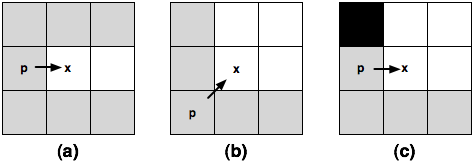
\includegraphics[width=0.95\columnwidth]
			{diagrams/pruning.png}
       \end{center}
	\vspace{-3pt}
       \caption{(a) When the move from $p$ to $x$ is straight only one natural neighbour remains.
(b) When the move from $p$ to $x$ is diagonal, three natural neighbours remain. (c) Obstacles around $x$
cause some neighbours to become forced. }
       \label{fig:pruning}
\end{figure}

We illustrate these rules in Figure~\ref{fig:pruning}(a) and ~\ref{fig:pruning}(b).
Observe that to test each rule we need to look only at
the neighbours of the current node $x$. 
Pruned neighbours are marked in grey. Remaining neighbours, marked
white, are called the \emph{natural} successors of node $x$.  
In Figure~\ref{fig:pruning}(c) we show
that obstacles can modify the list of successors for $x$:
when the alternative path $\pi' = \langle p, y, n \rangle$ is
not valid, but $\pi = \langle p, x, n \rangle$ is, we will refer to $n$ as
a \emph{forced} successor of $x$.
The set of forced successors in Figure~\ref{fig:pruning}(c) is different
to the set identified in~\cite{harabor11b}. 
In that work we assumed corner-cutting (a.k.a taking a diagonal shortcut around a corner) is allowed.
Here we explicitly require that both $\pi$ and $\pi'$ respect 
any such domain-specific movement rules.
When corner-cutting is not allowed this change has the following effect:
only straight steps from $p$ to $x$ may produce forced neighbours and each $x$ may have 
up to 4 such neighbours.
This change preserves optimality; the argument is identical to 
the one in~\cite{harabor11b}.

\textbf{Jumping Rules:}
JPS applies to each forced and natural neighbour of the current node $x$ a simple
``jumping'' procedure; the objective is to replace each neighbour $n$ with an 
alternative successor $n'$ that is further away. Precise details are given
in~\cite{harabor11b}; we summarise the idea here using a short example:

\begin{example}
In Figure~\ref{fig:pruning}(a) pruning reduces the number
of successors of $x$ to a single node $n$.
JPS exploits this property to immediately and recursively
explore $n$.
If the recursion stops due to an obstacle that blocks further progress
(which is frequently the case), all nodes on the failed path, including $n$, are ignored
and nothing is generated.
Otherwise the recursion leads to a node $n'$ which has a forced
neighbour (or which is the goal). JPS generates $n'$ as a successor of $x$; 
effectively allowing the search to ``jump'' from $x$ directly to $n'$ -- without adding
to the open list any intermediate nodes from along the way.
In Figure~\ref{fig:pruning}(b) node $x$ has three natural neighbours: two straight and one diagonal.
We recurse over the diagonal neighbour only if both straight neighbours produce
failed paths. This ensures we do not miss any potential turning points of the optimal path.
\end{example}

\begin{figure}[tb]
       \begin{center}
		   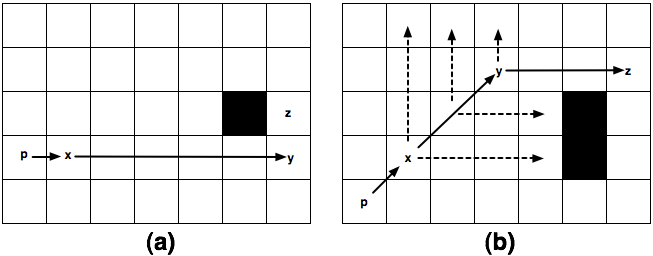
\includegraphics[width=0.95\columnwidth]
			{diagrams/jumping.png}
       \end{center}
	\vspace{-3pt}
       \caption{(a) A straight jump from $x$ to $y$; the recursion stops due to node $z$ which is forced.
(b) A diagonal jump from $x$ to $y$; the recursion stops due to a non-failed straight jump. Continuing 
would mean missing a potential turn due to $z$.}
       \label{fig:jumping}
\end{figure}

In Figure~\ref{fig:jumping}(a) we illustrate a straight jump and in \ref{fig:jumping}(b) a diagonal jump. 
By jumping, JPS is able to move quickly over the map 
without inserting nodes in the A* open list.
This is doubly beneficial as (i) it reduces the number of operations 
and (ii) it reduces the number of nodes in the queue, 
making each queue operation cheaper.  
Notice that this version of JPS is performed entirely online, involves no preprocessing and has no memory overhead.  


\chapter{Introduction}
\label{cha::intro}

Pathfinding is the name given to a broad class of related problems
often appearing in Computer Science. In the canonical case the
pathfinding problem asks that we navigate between an arbitrary pair of 
start and target locations drawn from a map. Such problems
appear in a myriad of important and real-life contexts. For example:
\begin{itemize}
\item Pathfinding is at the heart of all personal GPS navigation devices.
\item Pathfinding is used by transportation and logistics companies to 
improve performance and reduce operating costs.
\item Pathfinding is central to the correct operation of personal and industrial robots.
\item Pathfinding powers the AI systems of many modern computer games.
\end{itemize}

\noindent Just as there are many possible application areas for pathfinding there are
equally many variations of the problem as well. Frequently we are
asked to find a path which is optimal with regard to distance. In other cases
a more desirable path can be one that minimises travel time or even travel
cost.  Sometimes it may not necessary -- or even possible -- to compute an
optimal path: low-power or real-time computing devices place
strict limits on the amount of resources (CPU, memory) that are available for
navigation.  In these cases near-optimal, bounded sub-optimal or indeed any
path at all will often suffice. Other types of pathfinding problems include
(but are not limited to) finding a path in a dynamic environment, finding a path 
in three or more dimensions, navigating in the presence of other moving entities and
even chasing a moving target. All these topics have received 
extensive attention from both researchers and industrial practitioners.

In this thesis we will aim to compute distance-optimal paths in a discrete
and static two-dimensional environment. Our target applications are robotics and computer games.
We will study a range of different approaches but in each case our objective will
be (i) to find the shortest path, (ii) as quickly as possible and (iii) as economically
as possible with respect to available resources such as memory and pre-computation time. 


%\section{JPS+}
Jumping from one point to another in the grid avoids many unnecessary A* open
list operations and, as we will show in Section~\ref{cha::jps::results}, can
dramatically improve the performance of online pathfinding search.
Identifying these jump points often requires inspecting large sections of the
grid checking for forced neighbours. Though such operations usually take very
little time the procedure is nevertheless a bottleneck for the algorithm.  In
this section we develop JPS+: a variant of Jump Point Search which
pre-processes the map and replaces each adjacent neighbour of a grid node with
a jump point that lies in the same relative direction. The result of the
pre-processing is an adjacency list data structure that allows computing the
jump point successors of arbitrary nodes in constant time.


\begin{figure}[tb]
       \begin{center}
		   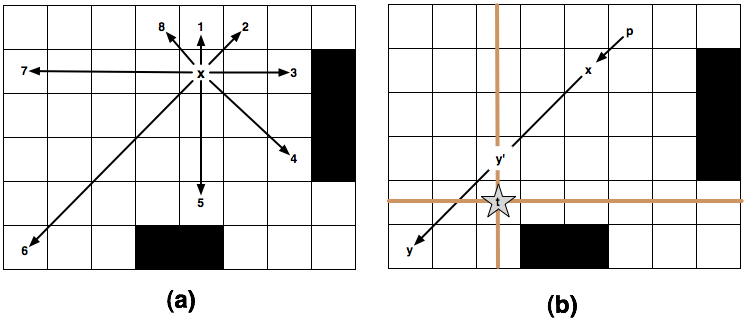
\includegraphics[width=0.95\columnwidth]
			{chapter_jps/diagrams/preproc.png}
       \end{center}
	\vspace{-3pt}
       \caption{(a) A jump point is computed in place of each grid neighbour of node $x$.
		(b) When jumping from $x$ to $y$ we may cross the row or column of the target $t$ (here, both). 
To avoid jumping over $t$ we insert an intermediate successor $y'$ on the row or column of $t$ (whichever is closest to $x$).}

       \label{fig:preproc}
\end{figure}

Figure~\ref{fig:preproc}(a) illustrates our graph reformulation idea for a 
single node $x$. We simply search for a jump point in the direction
of each grid neighbour of $x$. In JPS, we discard all nodes along a failed
path. By comparison, JPS+ must store the last node along a failed path.
These \emph{sterile jump points} are required 
to guarantee optimality during search but are never added to the A* open list.
To see why they are necessary, consider Figure~\ref{fig:preproc}(b).
Here we reach $x$ from $p$ and try to jump from $x$ to $y$. 
Notice that each such jump may cross the goal or column of the target node
$t$. In JPS the diagonal recursion would have terminated at node $y'$, having detected
the goal $t$ along a non-failed straight jump.
JPS+ simulates this behaviour by explicitly inserting an intermediate node $y'$ 
at the point where the jump to $y$ crosses the column of $t$.
This condition is sufficient to preserve optimality during search. The proof
involves showing that JPS+ simulates exactly the behaviour of JPS. We omit it 
for brevity.

\subsection{Properties}
JPS+ requires an offline pre-processing step that has quadratic time complexity
and linear space requirements w.r.t the number of nodes in the grid.



\begin{algorithmic}
\STATE {\bf input}: Graph $G$, source $s$, target $t$
\STATE $open := \{s\}$
\LOOP
  \STATE $i := pop(open)$
  \IF{$i = t$}
    \STATE {\bf return} $i$
  \ENDIF
  \IF{$i$ is a node}
    \FORALL{$i' \in$ successors\_of\_corner($i$)}
      \STATE add\_edge($i$,$i'$)
    \ENDFOR
  \ELSE %\COMMENT{$i$ is an interval}
    \STATE {\bf let} $i = \langle [x_{\min},x_{\max}],y,p\rangle$.
    \STATE $i_1 :=$ move($i$)
    \STATE $cs :=$ corners\_of($i_1$)
    \COMMENT{Including target.}
    \STATE $is :=$ split($i_1,cs$)
    \FORALL{$c' \in cs$}
      \IF{$c'$ is visible from $p$}
        \STATE add\_edge($i$,$c'$)
      \ENDIF
    \ENDFOR
    \FORALL{$i' \in is$}
      \STATE {\bf let} $i' = \langle [x'_{\min},x'_{\max}],y',p\rangle$.
      \IF{$\langle \frac{x'_{\min}+x'_{\max}}{2},y'\rangle$ is visible from $p$}
        \STATE add\_edge($i$,$i'$)
      \ENDIF
    \ENDFOR
  \ENDIF
\ENDLOOP
\end{algorithmic}


%\chapter{Conclusion}
\label{cha:conc}
Summary your thesis and discuss what you are going to do in the future in Section~\ref{sec:future}.


\section{Future Work}
\label{sec:future}
Good luck.





%%%%%%%%%%%%%%%%%%%%%%%%%%%%%%%%%%%%%%%%%%%%%%%%%%%%%%%%%%%%%%%%%%%%%%
% Here begins the end matter

%%% \appendix

\backmatter

\bibliographystyle{anuthesis}
\bibliography{references}

\printindex

\end{document}
